\documentclass[10pt,a4paper]{article}

\usepackage{graphicx}
\usepackage{amsmath}
\usepackage{float}
\usepackage{siunitx}
\usepackage{subcaption}
\usepackage{longtable,tabularx}
\usepackage{color}
\usepackage{pdflscape}
\usepackage{geometry}
\geometry{a4paper,left=25mm,top=40mm}
\newcommand{\indentitem}{\setlength\itemindent{25pt}}
\begin{document}
\begin{titlepage}
\centering

\vspace*{4cm}
{\huge\bfseries Agile Wing Integration Framework\par}

\vspace{1.5cm}
{\LARGE University of Bristol}

\vspace{0.5cm}
{\LARGE Future Projects Office}
\vfill
created by\par
Mr Christopher \textsc{Szczyglowski} (UoB)

Dr Dario \textsc{Calderon} (UoB)

Dr Robert \textsc{Cook} (UoB)

Dr Christopher \textsc{Howcroft} (UoB)

Mr Philip \textsc{Rottier} (Mathworks Consulting Services)

\vspace{3cm}
\begin{tabular}{rl}
Current Version: & V 0.1 \\
Created on : & 07/2018 \\
Administator: & Mr Christopher \textsc{Szczyglowski} \\
 & christopher.szczyglowski@bristol.ac.uk \\
Software Compatability: & Windows Operating System \\
& MATLAB version 2015b or later
\end{tabular}


\end{titlepage}

\section*{Disclaimer}
THIS SOFTWARE IS PROVIDED BY THE COPYRIGHT HOLDERS AND CONTRIBUTORS "AS IS" AND ANY EXPRESS OR IMPLIED WARRANTIES, INCLUDING, BUT NOT LIMITED TO, THE IMPLIED WARRANTIES OF MERCHANTABILITY AND FITNESS FOR A PARTICULAR PURPOSE ARE DISCLAIMED. IN NO EVENT SHALL THE COPYRIGHT OWNER OR CONTRIBUTORS BE LIABLE FOR ANY DIRECT, INDIRECT, INCIDENTAL, SPECIAL, EXEMPLARY, OR CONSEQUENTIAL DAMAGES (INCLUDING, BUT NOT LIMITED TO, PROCUREMENT OF SUBSTITUTE GOODS OR SERVICES; LOSS OF USE, DATA, OR PROFITS; OR BUSINESS INTERRUPTION) HOWEVER CAUSED AND ON ANY THEORY OF LIABILITY, WHETHER IN CONTRACT, STRICT LIABILITY, OR TORT (INCLUDING NEGLIGENCE OR OTHERWISE) ARISING IN ANY WAY OUT OF THE USE OF THIS SOFTWARE, EVEN IF ADVISED OF THE POSSIBILITY OF SUCH DAMAGE.

\section*{Release Statement}
This software is in the pre-alpha development stage meaning that perfect performance is not guaranteed. It is highly likely that there are many bugs remaining in the code and it is probable that the framework may not be compatible with all MATLAB versions and Airbus FAME models. In the event of an unexplained error the user is requested to inform the developers of the framework, providing sufficient detail (barring commercially sensitive information) such that the error can be replicated and solved.

\newpage
\tableofcontents

\newpage
\addcontentsline{toc}{section}{Introduction}
\section*{Introduction}

Agile Wing Integration (AWI) is an interactive environment for nonlinear aeroelastic analysis and preliminary sizing of conventional and unconventional aircraft configurations. The software is written entirely in object-orientated MATLAB code and requires a valid installation of MATLAB (version 2015b or later) to be executed. 

\parindent=0pt The framework comprises of several modules which are broadly split into three functional areas:


\begin{itemize}

\item \textbf{Importing Data} - The AWI framework supports the import of data from various file types. Information about the model and/or results data can be provided in Excel format (.xlsx), Comma-Separated-Variable (.csv), Extensible Markup Language (.xml) as well as MATLAB’s proprietary file format (.mat). AWI also supports the import of Airbus aircraft models and aeroelastic/sizing data from a FAME file (.fm4) as well as models designed using the CPACS parameterisation scheme. Further information on the data import process can be found in Section...

\item \textbf{Analysing Models} - The AWI framework supports various types of aeroelastic analysis, including:

\begin{itemize}

\item \textbf{Static Aeroelastic Trim} - Including automatic calculation of the optimum control surface deflection for a given trim case. 

\item \textbf{Dynamic Aeroelasticity} - Including ‘1-minus cosine’ and continuous turbulence analysis. 

%\item \textbf{Aeroelastic Stability Analysis} – Including classical flutter analysis and nonlinear continuation %analysis. 

\item \textbf{Additional Analyses} - Further analysis types are available within AWI, including the calculation of mass and inertia properties.

\end{itemize}

\item \textbf{Visualising and Exporting Data} - The AWI framework can also be used as a means of viewing and/or exporting results and model data.  Various methods are available for viewing results quantities, including: line plots, quiver plots, deformations and animations. Furthermore, the data in an AWI session can be exported to several formats:

\end{itemize}

AWI has been developed as a research tool by staff from the Aerospace Engineering Department at the University of Bristol (UK) in collaboration with Mr Philip Rottier of MathWorks Consulting Services. There are two intended user groups for the AWI framework:

\begin{itemize}
\item \textbf{University researchers}
\item \textbf{Aerospace engineers}
\end{itemize}

\section*{Getting Started}

\section*{Importing Data}

\section*{Analysing Models}

\section*{Viewing Results}

\section*{Exporting Data}

\section*{Method Description}

\section*{Code Description}

\addcontentsline{toc}{section}{Quick Start Guide (Airbus)}
\section*{Quick Start Guide (Airbus)}

This guide is intended as a brief introduction to the AWI framework. This guide will explain how to:

\begin{itemize}
{\indentitem \item{Obtain the AWI framework files}}
{\indentitem\item{Start the AWI framework}}
{\indentitem\item{Import a FAME aircraft model into the AWI framework}}
{\indentitem\item{Make changes to the model}}
{\indentitem\item{Run an aeroelastic analysis}}
{\indentitem\item{View results}}
{\indentitem\item{Export results}}
\end{itemize}

This document is a step-by-step guide of how to interact with AWI via the GUI. It will not discuss how to run AWI programmatically although this is arguably the more powerful use of the framework. 

There are two guides in this document:
\begin{enumerate}
{\indentitem\item A written guide that provides the bare minimum of detail and should be used as a prompt for users who are familiar with AWI.}
{\indentitem\item An annotated guide that uses screenshots to explain each step of the process. User’s who are unfamiliar with AWI should use this guide to help them get started.}
\end{enumerate}

Some assumptions are made about the user and the machine that they are working on. These assumptions are:

\begin{itemize}
{\indentitem\item The user is an employee of Airbus and has a working knowledge of the FAME-W analysis tool}
{\indentitem\item The user’s machine is running on a Windows operating system}
{\indentitem\item The user has already downloaded and installed a valid installation of MATLAB which is version 2015b or later.}
{\indentitem\item The user understands how to open MATLAB and run a file.}
\end{itemize}

\subsection*{Accessing the AWI files}

The source files for AWI are stored on the Airbus iShare portal. Mr Sylvain Boye\footnote{Sylvain Boye is a member of Airbus FPO, Filton, UK. Contactable at sylvain.boye@airbus.com} is the owner of the iShare and should be contacted if access is required. The files are stored at $<$INSERT FOLDER PATH HERE$>$ Simply download the .zip and extract the files to a folder location of your choice. 

At this point it is important that the user understands that the copy of the AWI framework that is held by Airbus is not version controlled. This has two main implications:
\begin{enumerate}
{\indentitem\item If any changes are made to the source files on the user’s machine they will be localised to the user’s machine, i.e. changes will not be propagated back to the iShare. The Airbus iShare is not a version-control system and the code available on the iShare is to be considered constant between any updates from the developers at the University of Bristol.}
{\indentitem\item Any changes that the user makes to the source files will cause a divergence in the codebase away from the version-controlled (original) code held by the University of Bristol. Therefore, it is not recommended that the user make any changes to the AWI source code as this will cause the software to become unreliable and will make debugging any issues very difficult. In future releases the source code may be obfuscated (p-coded) and released as a MATLAB package to protect the integrity of the AWI framework.}
\end{enumerate}

Written Step-by-Step Guide
\begin{enumerate}
%%%%%%%%%%%%%%%%%%%%%%%%%%%%%%%%%%%%%% START MATLAB
	\item \textbf{Start MATLAB}
	\begin{enumerate}
		\item Launch MATLAB via the Windows start-menu or using a desktop shortcut.
	\end{enumerate}
%%%%%%%%%%%%%%%%%%%%%%%%%%%%%%%%%%%%%% NAVIGATE TO THE AWI FILE LOCATION
	\item \textbf{Navigate to the AWI file location}
	\begin{enumerate}
		\item Use the folder browser on the left-hand side of the MATLAB window to navigate to the folder where the AWI files are located. 
	\end{enumerate}
%%%%%%%%%%%%%%%%%%%%%%%%%%%%%%%%%%%%%% START AWI
	\item \textbf{Start AWI} 
	\begin{enumerate}
		\item Type ``AWI'' in the MATLAB Command Window and press ``Enter'' to start AWI.
	\end{enumerate}
%%%%%%%%%%%%%%%%%%%%%%%%%%%%%%%%%%%%%% IMPORT A FAME MODEL
	\item \textbf{Import a FAME model} 
	\begin{enumerate}
		\item Using the menu-strip at the top of the GUI select File$\rightarrow$Import. (N.B. Previously imported models can be imported using File$\rightarrow$Reimport)
		\item Using the file selection window, navigate to the location of the FAME model that you wish to import, select the .fm4 file and click ``Open''. (N.B. Make sure the file specification is set to ``FAME Input files (*.fm4)'' using the drop-down menu above the ``Open'' button)
		\item If the import is successfully initialised a progress window will open which provides details of the actions being performed. These messages can be reviewed later by viewing the AWI ``Audit Trail''. This can be done by selecting Audit trail$\rightarrow$Show in the menu strip at the top of the GUI.
		\item Once the import process is complete the progress window will close, and a drawing of the model will be shown in the GUI. At this point, the user is free to view different aspects of the model, interrogate the model properties and make any necessary changes. Further details are provided in the Annotated Step-by-Step Guide.
	\end{enumerate}
%%%%%%%%%%%%%%%%%%%%%%%%%%%%%%%%%%%%%% MAKE CHANGES TO THE MODEL
	\item \textbf{Make changes to the model}
	\begin{enumerate}
		\item Changes to the model are made using the ``Property View'' which is accessible in two ways:
		\begin{enumerate}
			\item Through the object context menu
			\begin{itemize}
				\item Using the ``Tree View'' on the left-hand side of the AWI GUI, select the object you wish to edit, right-click to bring up the context menu and then navigate to Edit $\rightarrow$ Properties $\rightarrow$ This.  
				\item This version of the Property View is not dynamic, therefore the user is required to select ``Apply'' to propagate changes to the model which will then trigger a rebuild.
			\end{itemize}
			\item Through the GUI context menu
			\begin{itemize}
				\item Right-click on any of the top-level tabs in the GUI and select Add View $\rightarrow$ Properties.
				\item This version of the Property View is dynamic, meaning that any changes are automatically propagated to the model which is then rebuilt in real-time. 
			\end{itemize}
		\end{enumerate}
		\item The user should exercise caution when making changes as it is possible to drastically modify the model and cause a disparity between the geometry and the underlying structural properties of the model which has serious implications for the aeroelastic analysis and aircraft sizing modules.
	\end{enumerate}
%%%%%%%%%%%%%%%%%%%%%%%%%%%%%%%%%%%%%% RUN AN AEROELASTIC ANALYSIS
	\item \textbf{Run an aeroelastic analysis}
	\begin{enumerate}
		\item To run an aeroelastic analysis the AWI session must contain a valid aircraft model and at least one valid load case. Furthermore, when analysing FAME models, the user must have imported the FAME results data containing the aircraft mass and stiffness distribution.
		\item \textbf{Running an aeroelastic trim analysis}
		\begin{enumerate}
			\item To initiate an aeroelastic trim analysis select Analyse $\rightarrow$ Aeroelastic $\rightarrow$ Trim using the menu strip at the top of the GUI.
			\item Selecting this option will automatically open a new view in the GUI called ``TrimAnalysis''. 
			\item Using the drop-down menu on the right-hand side of the new view, select the load case and beam model for analysis by the trim solver \footnote{A beam model defines the various mass and stiffness properties of the aircraft. Multiple beam models may be present in the AWI session if the user has run a sizing analysis or has imported multiple FAME models.}. 
			\begin{itemize}
				\item N.B. The user is automatically given the option of all available ``manoeuvre'' load cases in the AWI session. If, for some reason, there are no load cases of type ``manoeuvre'' then the user will be unable to run a trim analysis.
			\end{itemize}
			\item Select ``Trim…'' to run the trim solver. N.B. By default the trim solver will use the aircraft pitch angle and the elevator to balance the aircraft weight and pitching moment.
			\item Whilst the trim solver is running the user can monitor the progress of the solution and view the state of the model, including: the residual norm, the aircraft deflections and the control surface deflections.
			\item Once the trim solver has achieved convergence the TrimAnalysis view will be populated by some preliminary results and a new result set will be added to the AWI session.  This can be viewed in the tree view by expanding the ``Results Sets'' node and looking under the relevant beam model.
		\end{enumerate}
		\item \textbf{Running a 1-minus cosine gust analysis}
		\begin{enumerate}
			\item To initiate a 1-minus cosine analysis select Analyse $\rightarrow$ Aeroelastic $\rightarrow$ Gust using the menu strip at the top of the GUI.
			\item Selecting this option will automatically open a new view in the GUI called ``GustAnalysis''. 
			\item Using the drop-down menu on the right-hand side of the new view, select the load case, beam model and the trim result for analysis by the gust solver.
			\begin{itemize}
				\item N.B. The user is automatically given the option of all available ``one-minus-cosine'' load cases in the AWI session. If, for some reason, there are no load cases of type ``one-minus-cosine'' then the user will be unable to run a gust analysis.
				\item A trim result is required to allow the gust solver to start the model from its deformed/trimmed shape. This represents an important difference from traditional linear tools as the case where nonlinearities are included the gust response is dependent on the initial conditions of the system, i.e. the initial trimmed shape.
				\item The trim condition will be calculated automatically if no trim result is present that matches the specified flight-point.
				\item If there are no ``one-minus-cosine'' load cases in the AWI session the user can create their own. For further details see the Annotated Step-by-Step Guide.
			\end{itemize}
			\item Select ``Analyse…'' to run the gust solver.
			\item Once the gust solver has finished the GustAnalysis view will be populated by some preliminary results and a new result set will be added to the AWI session.  This can be viewed in the tree view by expanding the ``Results Sets'' node and looking under the relevant beam model.
			\begin{itemize}
				\item As the gust analysis is a transient analysis there is a significant amount of data that is generated. These results are split into two categories:
				\begin{enumerate}
					\item \textbf{Static Results} - For every gust length considered, the maximum and minimum loads with respect to time are calculated for every spanwise position along each beam in the analysis model. These results are added to the ``Static Results'' collector in the tree view.				
					\item \textbf{Transient Results} - For every gust length considered, the raw time domain data is retained and added to the ``Transient Results'' collector in the tree view.
				\end{enumerate}
			\end{itemize}
		\end{enumerate}
	\end{enumerate}
%%%%%%%%%%%%%%%%%%%%%%%%%%%%%%%%%%%%%% VIEW RESULTS
	\item \textbf{View Results}
	\begin{enumerate}
		\item \textbf{Add a ``Beam Results Viewer'' view} - In order to view the results, the appropriate view must be added to the GUI. Right click on any of the top-level GUI tab pages to bring up the AWI View Manager context menu and select Add View $\rightarrow$ Beam Results Viewer.
		\begin{enumerate}
			\item \textbf{N.B.} The ``Static Results View'' shows results data which is independent of time. These results are either associated with manoeuvre load cases or are the maximum and minimum envelope loads from a gust analysis. The results viewer allows the user to view the distribution of a results quantity over the span of a beam, however, it will not show the user any time history data.
		\end{enumerate}	
		\item \textbf{Select the results} –  - 
		\begin{enumerate}
			\item \textbf{Results Sets (Multi-Select)} - A results set represents the output from a single analysis. The Beam Results Viewer allows quantities from multiple results sets to be viewed at once.
			\item \textbf{Beam Elements (Single-Select)} - After selecting a result set the user is offered a selection of all the common beam elements for which a results quantity has been defined. When considering results from a FAME model this will typically be just the starboard wing, however, if the user runs an aeroelastic analysis using the AWI framework then there will be results for other ``beams'' in the model such as the VTP, HTP, etc.
			\item \textbf{Results Types (Single-Select)}  - After selecting a result set and a beam element to view the results over, the user will be offered a choice of all results types in the chosen result set. A results type defines a group of results and is dependent on what type of result set has been selected. For instance, an aeroelastic result set will have various aerodynamic and structural results quantities defined, however, a sizing result will contain information about the box thicknesses etc. 
			\item \textbf{Results Quantities (Multi-Select)} - After selecting the results type the user will be offered a selection of all results quantities in this results type. The user is able to select any number of results
		\end{enumerate}
		\item \textbf{Customise the display}
		\item \textbf{Calculate the loads envelope}
	\end{enumerate}
%%%%%%%%%%%%%%%%%%%%%%%%%%%%%%%%%%%%%% EXPORT RESULTS
	\item \textbf{Export Results}
	\begin{enumerate}
		\item \textbf{Add a ``Static Results'' view} - An instance of the ``Static Results View'' is required to initiate the export process.
		\item \textbf{Select ``Export Results...''} - Click the ``Export Results…'' push button to open up the ``AWI Export Manager''.
		\item \textbf{Configure export specification} - The following options must be set before the results can be exported:
		\begin{enumerate}
			\item \textbf{Results Selection (Multi-Select)} - The export manager will honour the current selection of results sets, however, this is easily changed by the user if a different selection is required. Simply highlight the results in the list-box or click ``Select All'' to select all results sets.
			\item \textbf{Beam Elements (Multi-Select)} - The user must select the beams over which the results data is defined.
			\item \textbf{Results Types (Multi-Select)} - The user must select the results types to be exported. Every results quantity from the selected results types will be exported.
			\item \textbf{Export Directory} – The use must select a folder location for the results to be saved to. The full directory path can be pasted into the edit box or the user can click the `open' button to select a directory using the Windows Explorer.
			\item \textbf{Export File Format} - The user must select the format for exporting the results. The number of files that are generated is dictated by this option.
			\begin{itemize}
				\item \textbf{CSV (.csv)} - This option is much quicker but generates more files. One file is generated per results quantity (for each beam) and each file contains the data for that results quantity across all selected results sets.
				\item \textbf{Excel (.xslx)} - This option is slower and generates fewer files. One file is generated per results type and each results quantity is defined on a separate (named) sheet in the excel workbook. 
				\begin{enumerate}
					\item The slower speed is attributed to using MATLAB’s inbuilt `xlswrite' function as opposed to a vectorised call to `fprintf' which is what the csv-exporter uses.
				\end{enumerate}
				\item \textbf{N.B.} - The output files are automatically named based on the beam name and results type/quantity. If a file of the same name (and file extension) already exists in the export directory, then the new results will be appended to that file.
			\end{itemize}
		\end{enumerate}
		\item \textbf{Export the data} - Hit ``Export'' to initiate the export process. A progress dialogue box will open during the export process and will close once the last file has been written. 
	\end{enumerate}
\end{enumerate}
\subsection*{Annotated Step-by-Step Guide}

\newpage
\begin{landscape}
\subsubsection{Navigate to the AWI files and start AWI}
\end{landscape}

\newpage
\begin{landscape}
\subsubsection{The AWI GUI}
This is the AWI opening screen

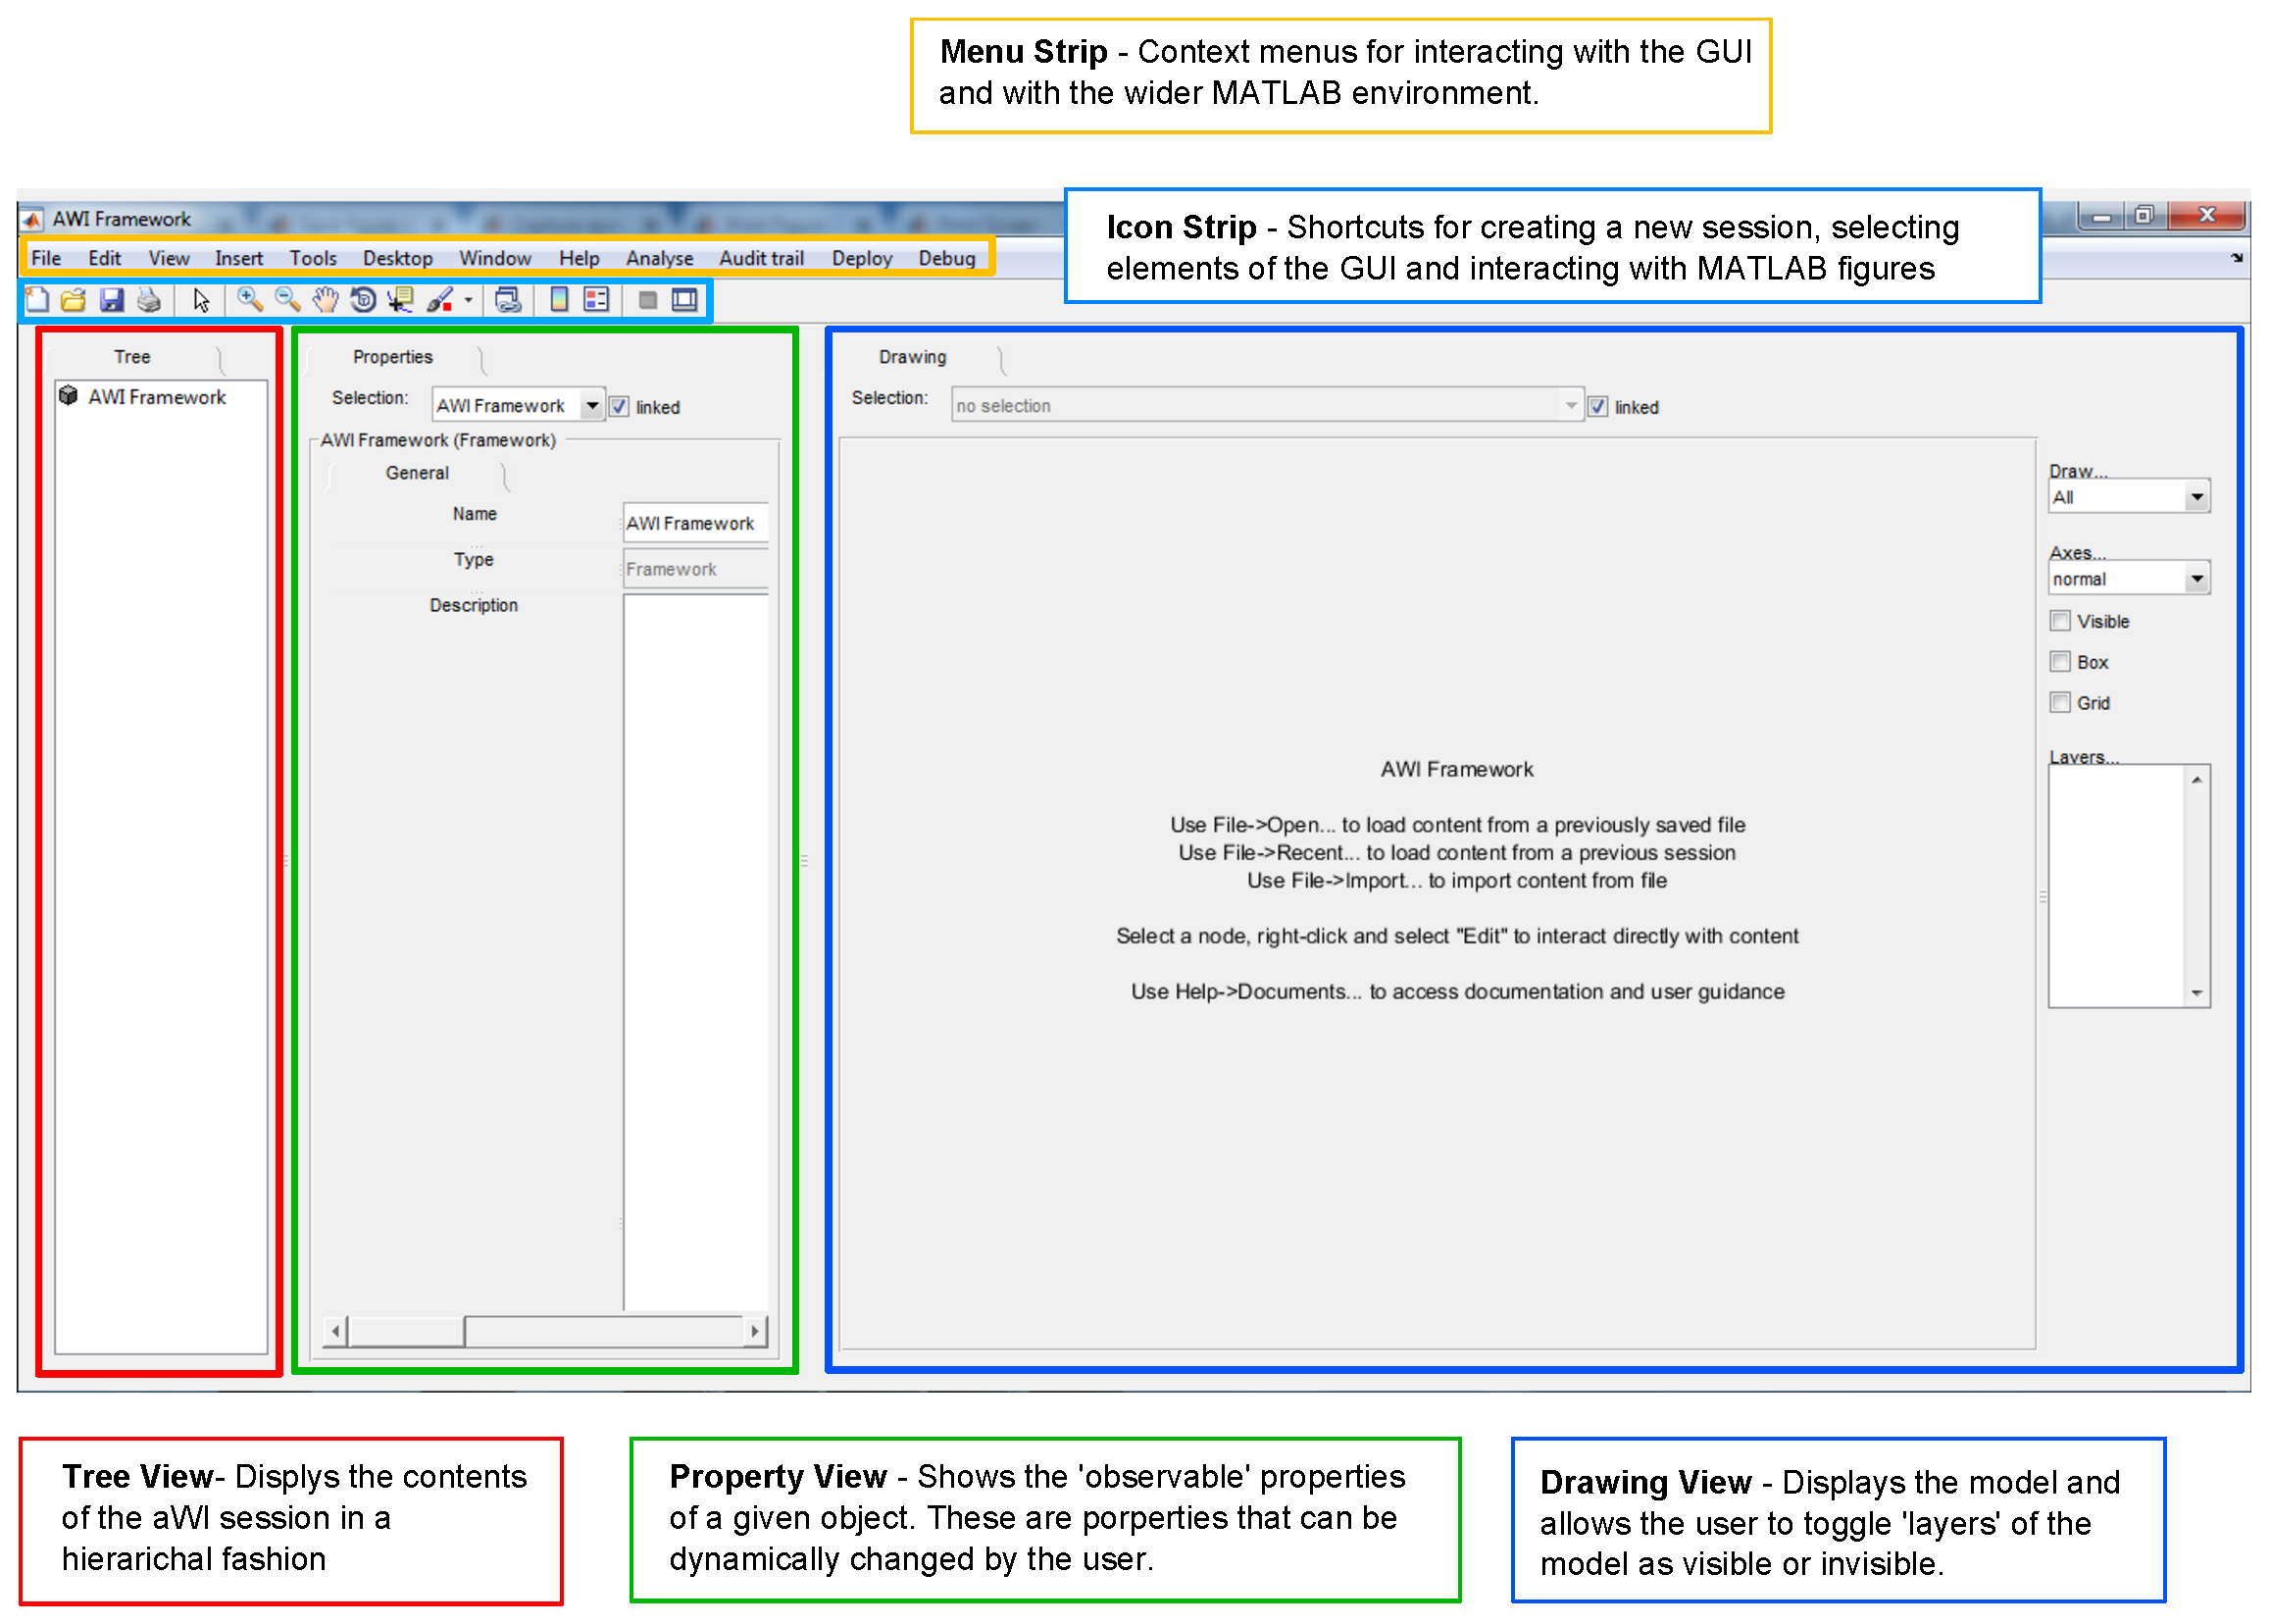
\includegraphics[width=1.3\textwidth]{AWIGUI.eps}
\end{landscape}

\newpage
\begin{landscape}
\subsubsection{Import a FAME model}
Using the menu strip, select File>Import to launch the file browser window. Navigate the FAME model that you wish to import and select the .*fm4 file.

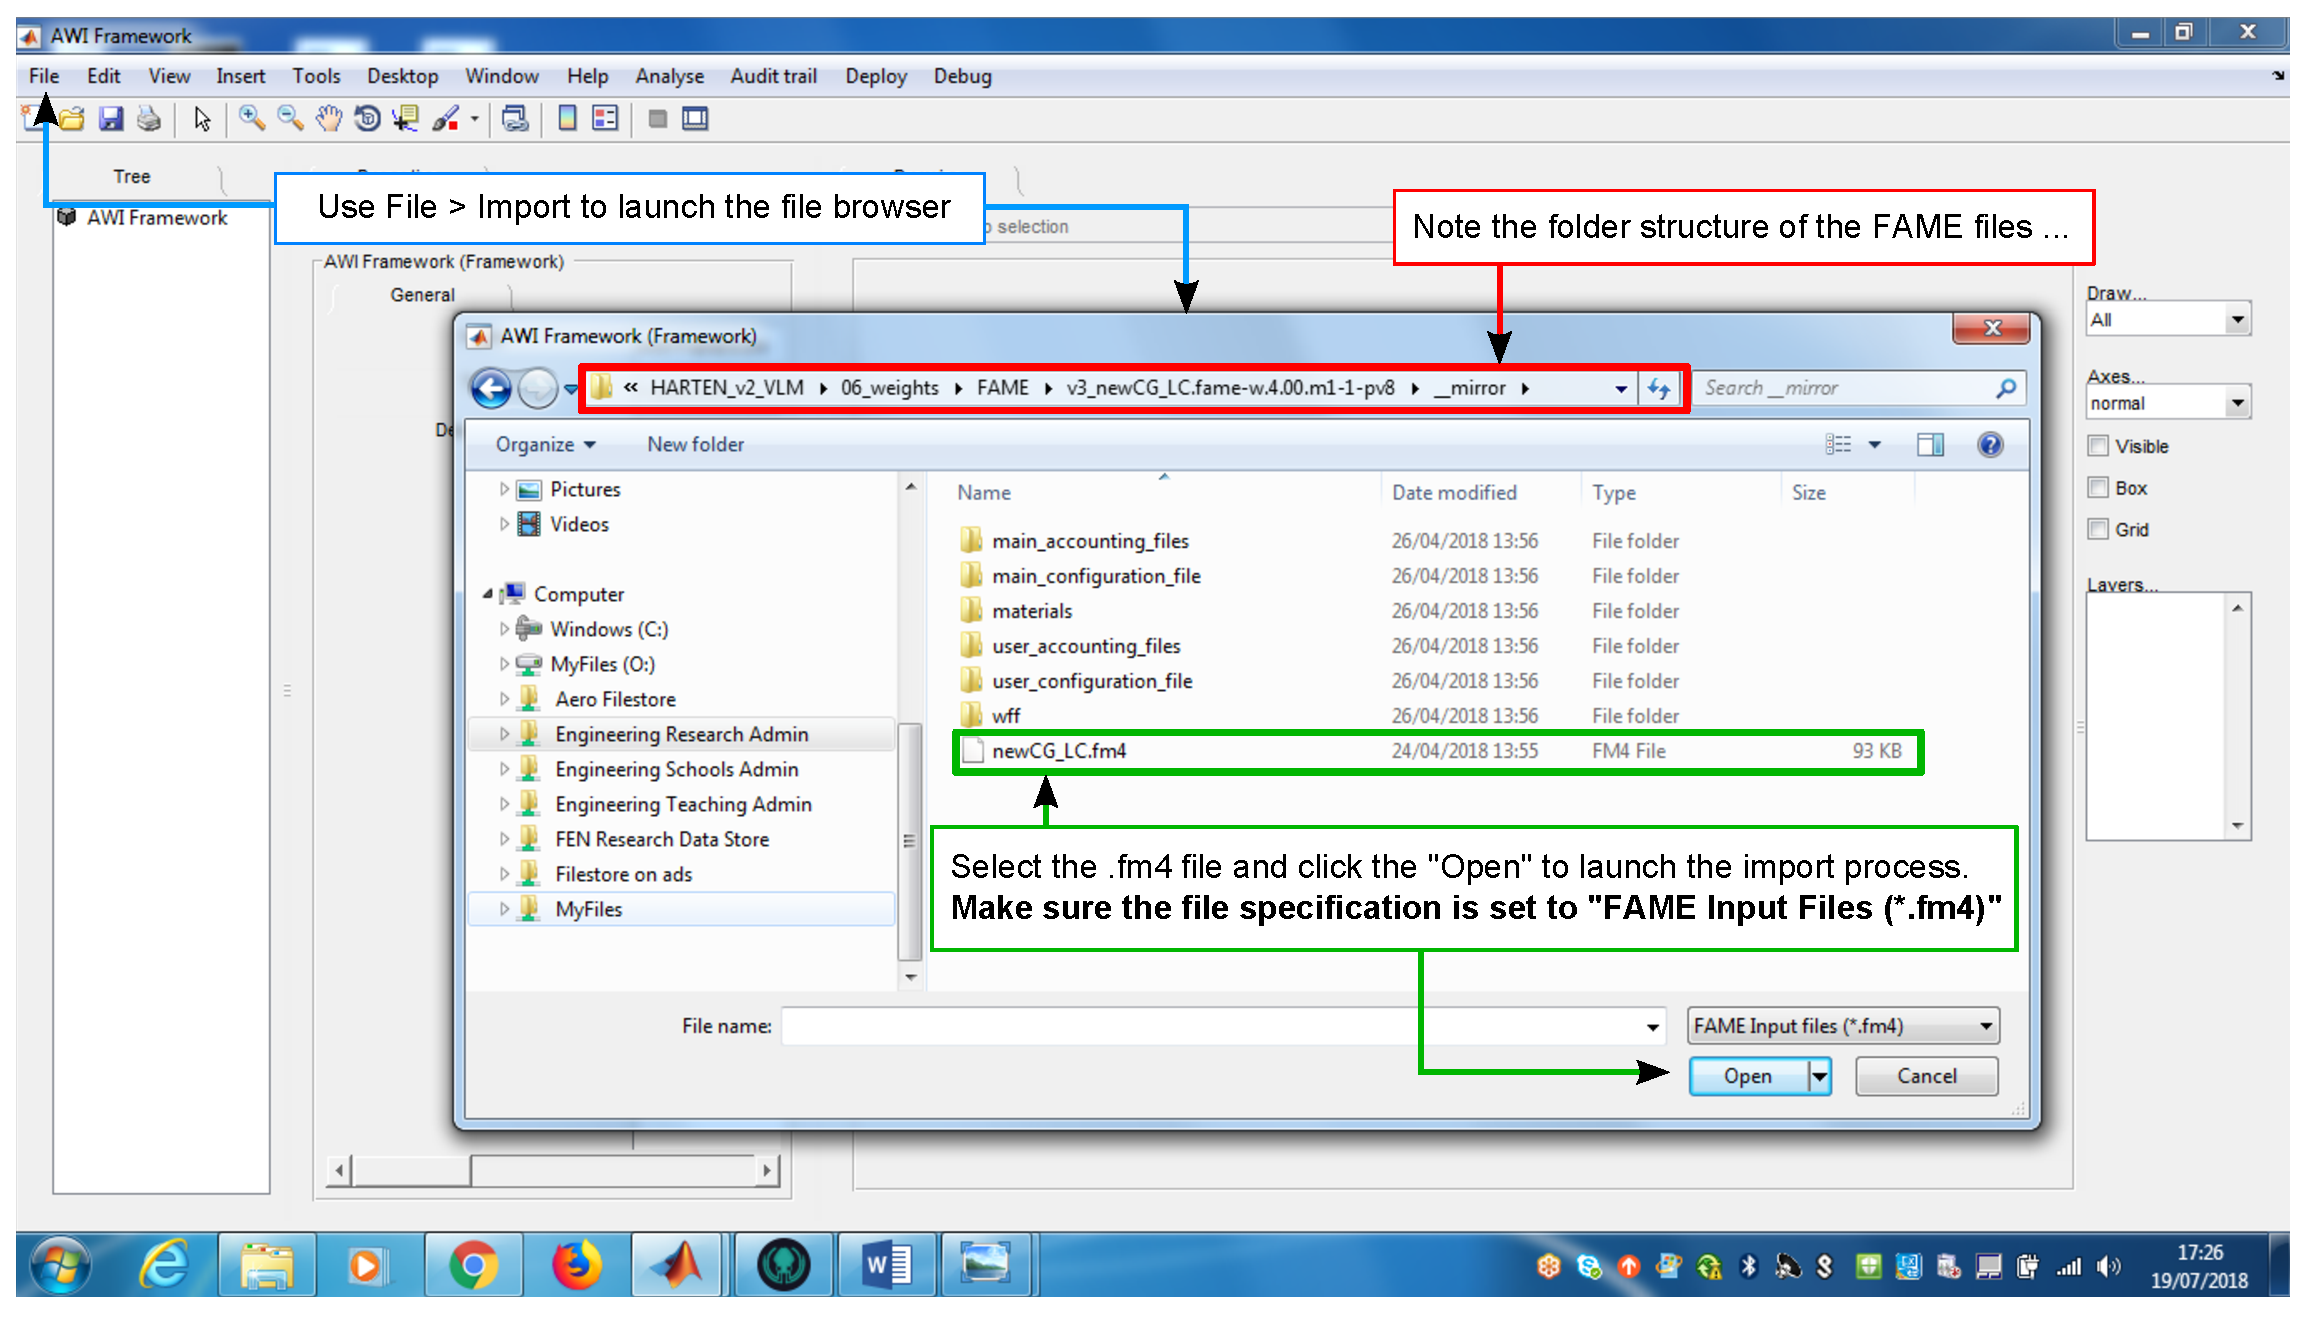
\includegraphics[width=1.3\textwidth]{ImportFame.eps}
\end{landscape}


\addcontentsline{toc}{section}{Converting FAME to AWI Workspace (Airbus)}
\section*{Converting FAME to AWI Workspace (Airbus)}
This section provides a discussion on: 
\begin{itemize}
\item The process through which the AWI framework is able to read and convert the FAME files into the MATLAB workspace
\item The assumptions made by the framework regarding which files are needed and where they are expected to exist in the available folder structure.
\end{itemize}
\addcontentsline{toc}{subsection}{Assumptions about the FAME folder structure}
\subsection*{Assumptions about the FAME folder structure}

An example of the type of folder structure expected by the AWI framework is presented in figure \ref{fig:FAMEFolderStructure}. It is important to note in most cases the framework will give the user the ability to locate the required files if it is not able to find them. File and folder requirements are discussed below.

\begin{enumerate}
	\item \textbf{Main entry point} - The main entry point to the FAME files is the \textbf{*.fm4} file. This is highlighted in blue in figure \ref{fig:FAMEFolderStructure}. The framework assumes that one of the parent folders of the fm4 file is labelled \textbf{`06$\_$weights'}. In the case where such a parent folder does not exist, the framework's assumed path structure will fail and will consequently request the user to find the required files as they are needed by the framework. Therefore, the assumed path structure is not critical but it is preferable. Currently, the \textbf{*.fm4} is expected to exist in the \textbf{$\_\_$mirror} folder as illustrated in figure \ref{fig:FAMEFolderStructure}. If the framework realises that $\_\_$mirror folder is not the immediate parent folder of the *.fm4 file, then it asks the user to select the main FAME output folder which is generally labelled \textbf{*-pv8}. A check is performed to ensure that the `$\_\_$mirror', `1$\_$structure', and 'export' folders exist in the newly selected FAME folder.
	\item \textbf{*tux$\_$xml file} - The `tux$\_$xml' file is expected to exist in a folder called \textbf{`01$\_$geometry'} at a similar level to where the `06$\_$weights' is found. If the framework fails to find this file it will ask the user to locate the file for it. This folder is used to extract geometries of the aircraft which may be missing from the fm4 file.
	\item \textbf{FAME results} - The fame results (deformations, internal loads, aerodynamic loads etc.) are expected in the \textbf{`*.m1-1-pv8/export/fmwpp01/flexible'} folder. If the results are not found then the import process will step out without looking for the following files:
	\begin{enumerate}	
		\item \textbf{Load Case file} - Information about the load cases are currently retrieved from the \textbf{`loadcase$\_$info.txt'} file, as it contains more information than is available in the fm4 file. It is assumed that this file is located in \textbf{`*.m1-1-pv8/1$\_$structure/1$\_$10$\_$wing/13$\_$fame-w/flexible'}. If the file is not found, the framework will ask the user to locate it.
		\item \textbf{Nastran files} - A nastran file which is generated by the FAME sizing process and contains GRID, PBAR, CBAR and MAT1 entries is currently used by the framework to discretise the wing in to a series of finite beam elements. The framework is only interested in the following file \textbf{`*.m1-1pv8/1$\_$structure/1$\_$10$\_$wing/13$\_$fame-w/flexible/deformations /model$\_$nastran$\_\_$ldcase0001.dat'}. The rest of the nastran files, containing the point loads associated to each load case are used to extract the loads and not the beam properties.
		\item \textbf{Wing mass files} - The framework assumes that the wing mass file is contained in the folder \textbf{`$\_\_$mon/wbd2/massdist/flexible'}. It expects files of the form `*.205'. In the case where it finds both an unsorted and sorted file (\textbf{massdist$\_$items.205} and \textbf{`massdist$\_$items $\_\_$sorted.205'}) the framework will prioritise the sorted file and extract both the primary and secondary masses.
		\item \textbf{Fuel mass files} - The fuel mass files are expected to exist in \textbf{`$\_\_$mon/wbd2/massdist/ flexible'}. Given that the naming of the fuel files are arbitrary and subject to the Airbus user, the framework currently performs a search criteria within that folder for any files with the name \textbf{`right*'}. If the framework is unable to find any files of that type, then it will ask the user to find the files. It is not critical to select all of the fuel files but preferable if all are selected, as the fuel mass closest to that specified in the loadcase will be assigned to the beam model later on in the aeroelastic analysis. 
	\end{enumerate}
\end{enumerate}
\begin{figure}[h!]
\centering
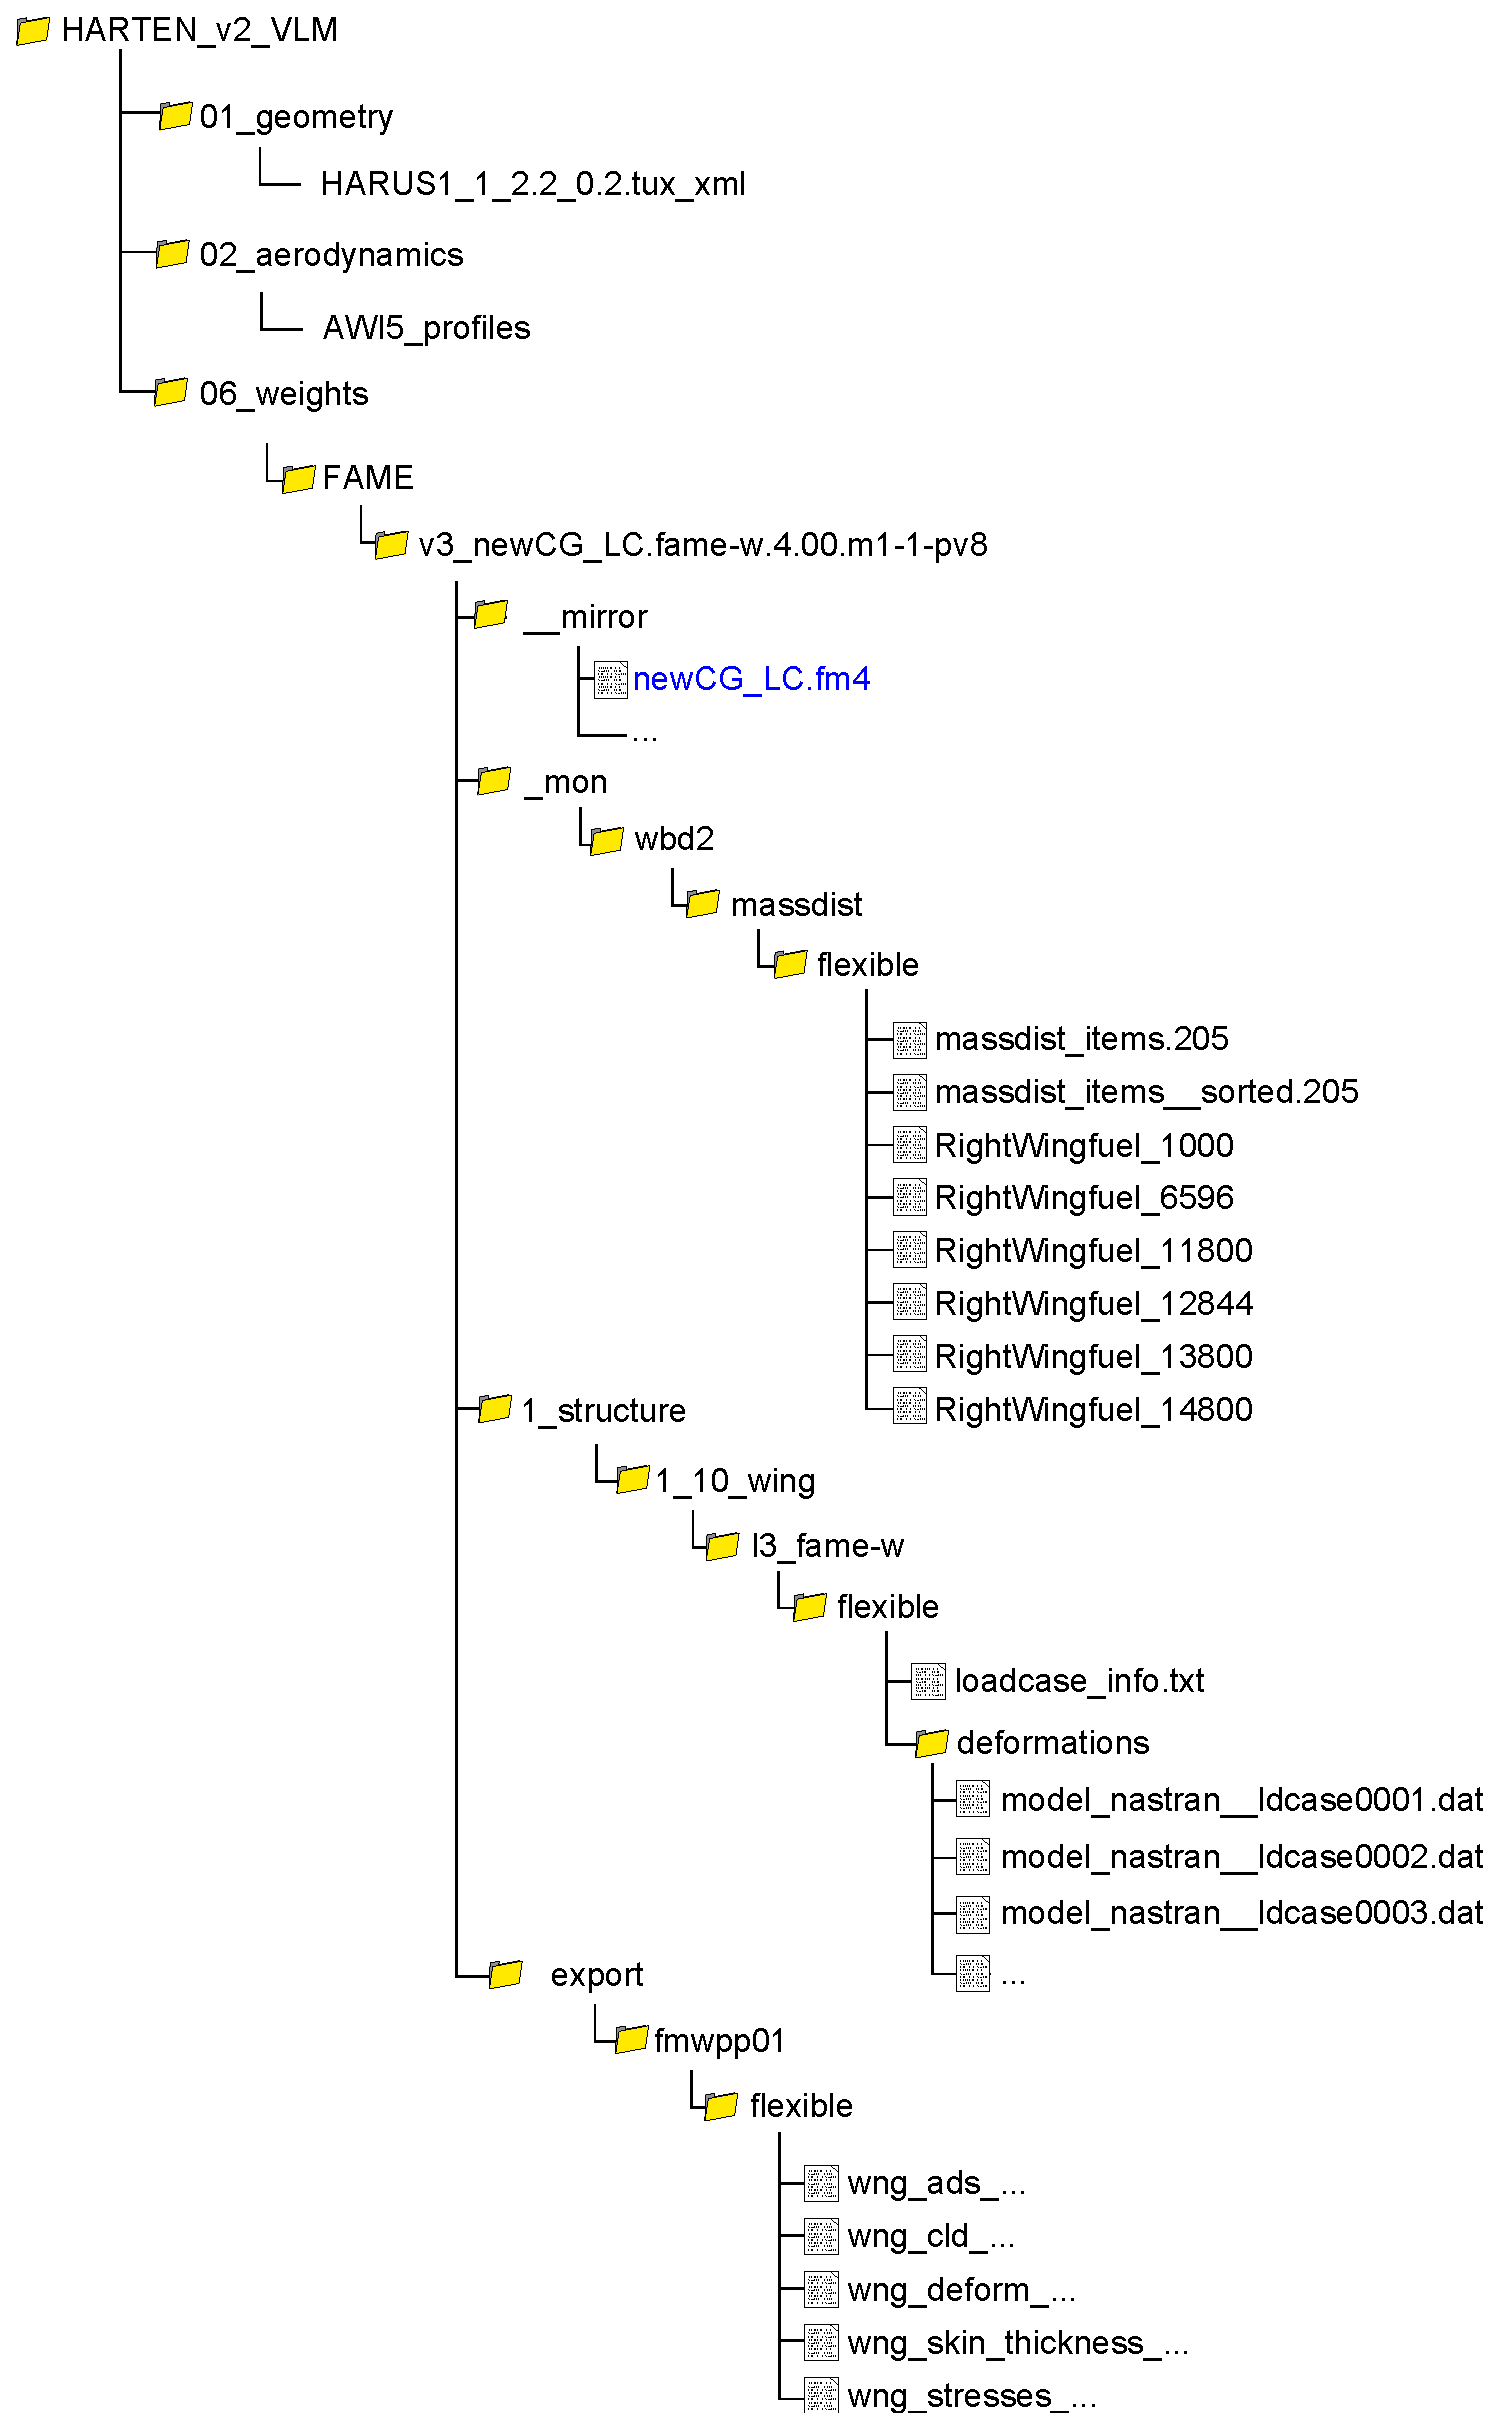
\includegraphics[width=0.7\textwidth]{FAMEFolderStructure}
\caption{FAME Folder Structure}\label{fig:FAMEFolderStructure}
\end{figure}

\addcontentsline{toc}{subsection}{An explanation on the FAME import procedures}
\subsection*{An explanation on the FAME import procedures}

\begin{enumerate}
\item \textbf{Read *fm4 file} - The first step in the FAME import process is to read and parse the input file into the MATLAB workspace. The underlying function ``getFameInput'' grabs all of the information found in this single file, and creates a structure array that preserves the structure in the file. \textbf{N.B.} It is important to note that the current version ignores `INCLUDE' entries in the file and therefore, pertinent information, which will be outlined further on, must be explicitly written into the .fm4 file. 

\item \textbf{Read *tux$\_$xml file} - The `tux$\_$xml' file is also used by the FAME file reader. Since FAME-W is a wing sizing tool, empennage geometries are usually omitted from the .fm4 file. The AWI framework circumvents this by extracting all of the information found in the tux file and isolating the `vtp' and `htp' entries to create the empennage geometries. An outline of the aerodynamic surfaces is created and later used to generate a finite element model. Control surfaces are added to the `vtp' and `htp'. Engine and fuselage geometries are also used by the AWI framework if they exist in the `tux$\_$xml' file.

\item \textbf{Read FAME results} - The FAME results are then extracted and stored internally.

\item \textbf{Read FAME Nastran File} - A nastran finite element model is automatically generated by the FAME sizing process and passed into the AWI framework. The beam elements in this file belong to the wing and contain stiffness properties which correspond to the 3-dimensional properties of the internal wing sections obtained through the FAME sizing. Figure \ref{fig:FAMENastranModel} illustrates the original beam model extracted from FAME.

\begin{figure}[h!]
\centering
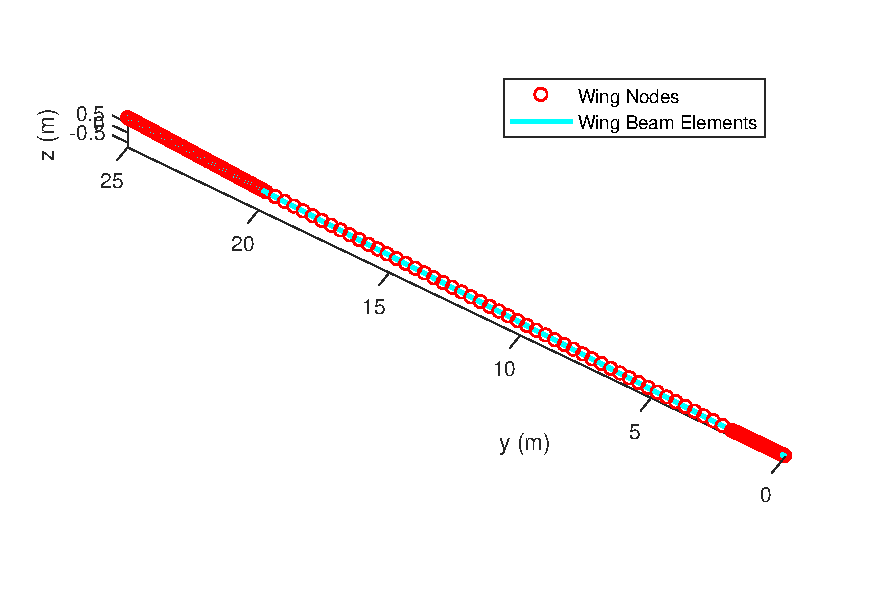
\includegraphics[width = 0.7\textwidth]{FAMENastranModel}
\caption{FAME Nastran finite element model}\label{fig:FAMENastranModel}
\end{figure}

\begin{figure}[h!]
\centering
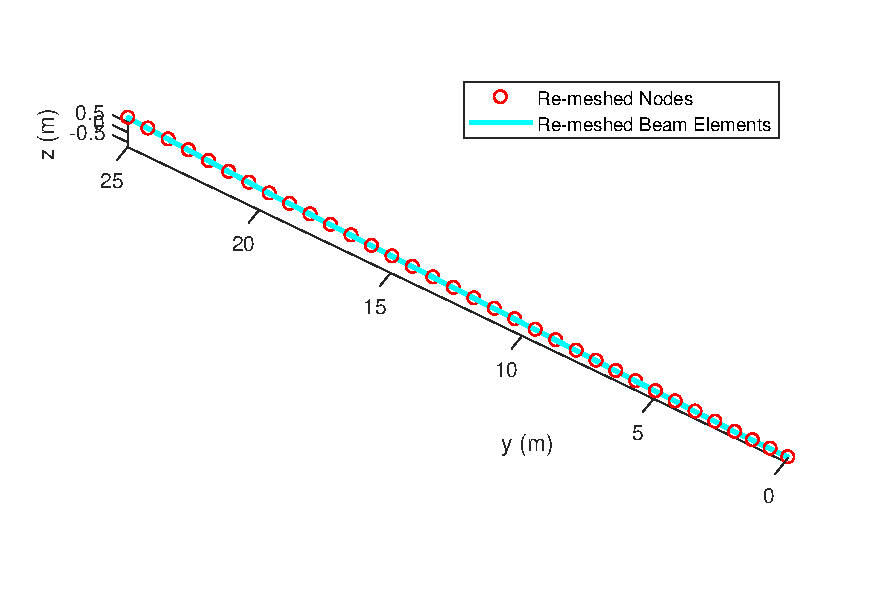
\includegraphics[width = 0.7\textwidth]{FAMENastranModelRe-meshed}
\caption{Reduced FAME finite element model}\label{fig:FAMENastranModelReduced}
\end{figure}

It is often the case that the FAME wing beam model is made up of a large number of beam elements ($>$150). In order to improve the simulation run time this beam model can be re-meshed. Currently, the re-meshing takes place during the import process and cannot be altered after the fact. However, the ability to arbitrarily discretise the beam model from within the framework will be added in a future version. An example of a beam model which has been reduced to 32 beam elements is shown in figure \ref{fig:FAMENastranModelReduced}. A comparison between the stiffness properties of the original and the reduced beam model is presented in figure \ref{fig:OriginalvsReducedStiffness}.

\begin{figure}[h!]
\centering
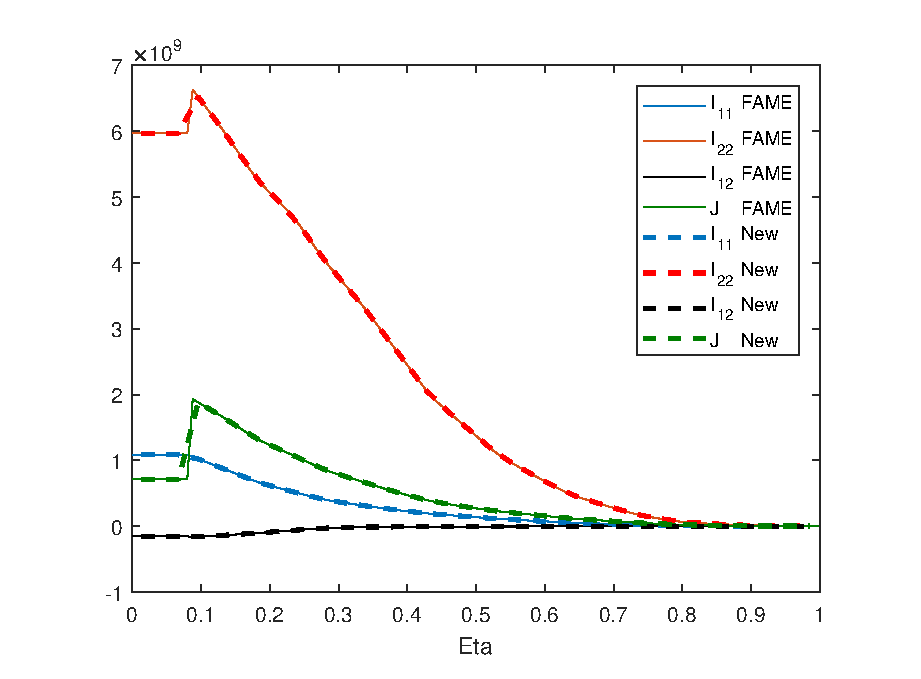
\includegraphics[width = 0.7\textwidth]{StiffnessComparison}
\caption{A comparison of the sectional properties of the FAME model, before and after model reduction}\label{fig:OriginalvsReducedStiffness}
\end{figure}

\item \textbf{Get Wing Masses} - The wing masses are extracted from the .205 file in the FAME folder. The process consists of retrieving the mass, centre of gravity and mass moment of inertia of each point mass and consolidating them onto a single lumped mass per node along the wing. Figure \ref{fig:OriginalFAMEMasses} illustrates the original masses taken from FAME and figure \ref{fig:ReducedFAMEMasses} shows the aggregation of these masses according to the reduced finite element model.

\begin{figure}[h!]
\centering
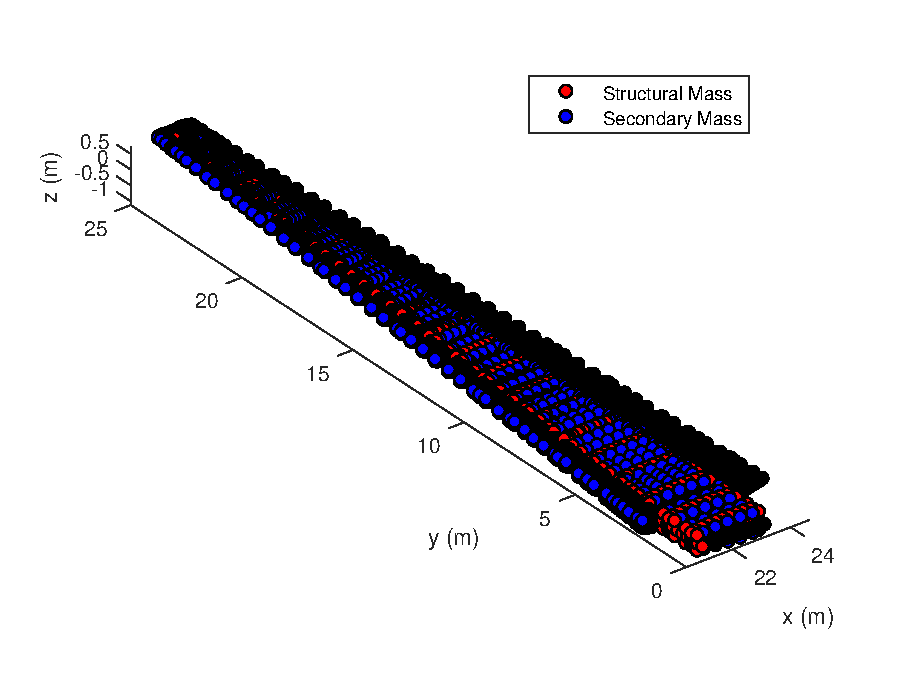
\includegraphics[width = 0.7\textwidth]{OriginalFAMEMasses}
\caption{FAME lumped masses representing primary and secondary masses}\label{fig:OriginalFAMEMasses}
\end{figure}

\begin{figure}[h!]
\centering
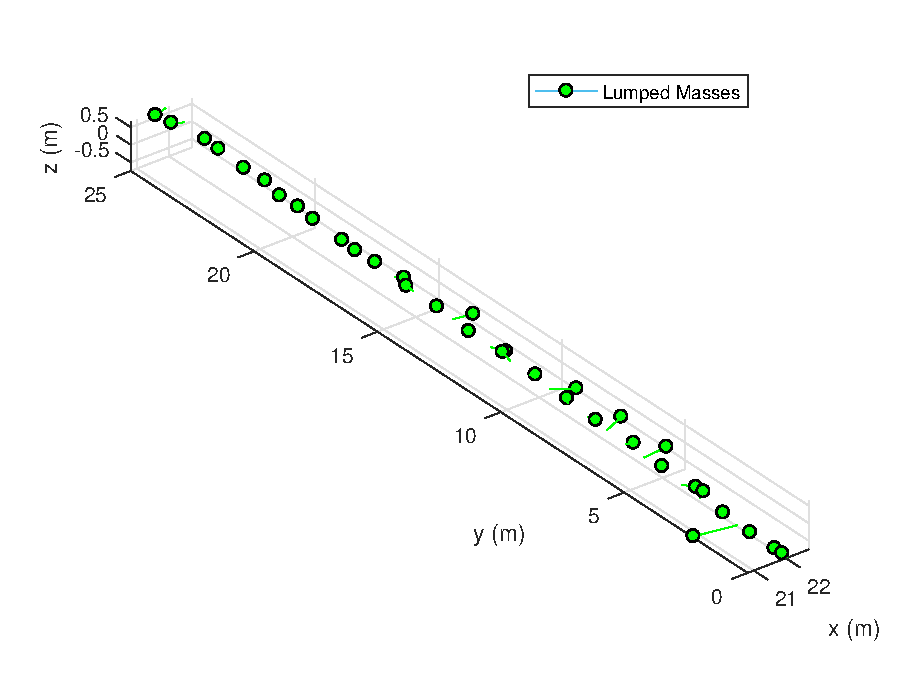
\includegraphics[width = 0.7\textwidth]{ReducedFAMEMasses}
\caption{Reduced FAME lumped masses for the primary and secondary mass}\label{fig:ReducedFAMEMasses}
\end{figure}

\item \textbf{Get Fuel Masses} - The fuel mass distribution is obtained from aformentioned user created files which contain point masses for each fuel configuration. The number of point masses is reduced in a similar manner to the wing mass. The fuel is stored separately and treated as a special mass which is associated to a particular load case. 

\item \textbf{Define additional masses} - In addition to the wing masses and the fuel masses the import process must assign mass to the rest of the aircraft. The empennage consists of rigid beam elements coupled to lumped masses to represent its mass. Given that the mass of the empennage is not specified anywhere in the FAME sizing process, an estimate is made. 

\begin{itemize}
\item \textbf{Engine} - If the engine is wing-mounted then the position and mass is directly transferred to the finite element model. If it is rear-mounted and defined in the tux$\_$xml file, then the engine mass is estimated and placed accordingly. 
\item \textbf{HTP} - The HTP mass is estimated at 0.9\% of the MTOW specified in the fm4 file.
\item \textbf{VTP} - The VTP mass is estimated at 1.4\% of the MTOW specified in the fm4 file.
\item \textbf{Fuselage} - The fuselage mass is estimated by ensuring that the lumped masses in the finite element model add up to the OEW. If the OEW is not specified anywhere in the FAME input files then it is estimated at 25\% of the MTOW specified in the fm4 file.
\end{itemize}

\item \textbf{Define aerodynamic surfaces} - Figure \ref{fig:FAMEAerodynamicSurface} illustrates the aerodynamic surfaces generated by the import process. The discretisation of the spanwise aerodynamic panels are chosen to match the beam elements, therefore, a one-to-one correspondance exists.  

\begin{figure}[h!]
\centering
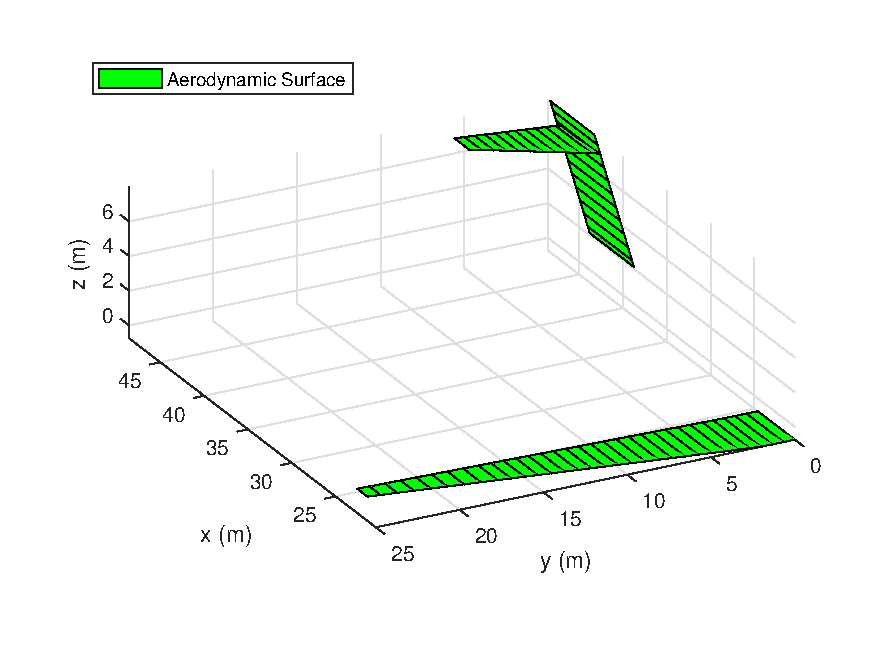
\includegraphics[width = 0.7\textwidth]{FAMEAerodynamicSurface}
\caption{Reduced FAME lumped masses for the primary and secondary mass}\label{fig:FAMEAerodynamicSurface}
\end{figure}

\item \textbf{Define aerodynamic nodes} - Figure \ref{fig:FAMEAerodynamicNodes} illustrates the aerodynamic nodes generated by the import process, which are then used to create interploation sets for the aerodynamic surfaces and the structural grids. 

\begin{figure}[h!]
\centering
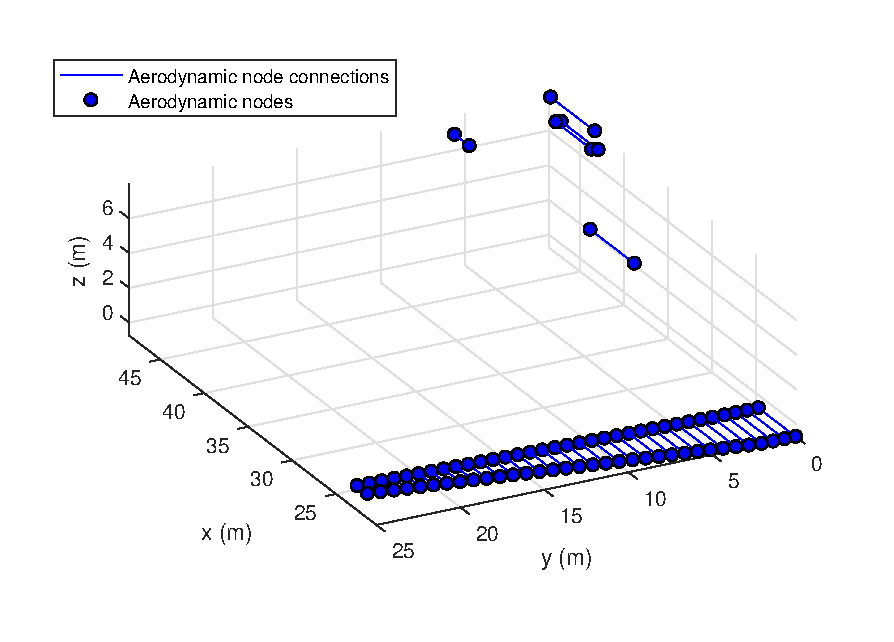
\includegraphics[width = 0.7\textwidth]{FAMEAerodynamicNodes}
\caption{Aerodynamic nodes and their corresponding connections, used for splining between aerodynamics surfaces and structural grid nodes}\label{fig:FAMEAerodynamicNodes}
\end{figure}

\item \textbf{Reflect the model} - Figure \ref{fig:ReflectedModel} illustrates the reflected aircraft model and figure \ref{fig:FAMEModelFramework} presents the users view of the imported model within the AWI GUI.

\begin{figure}[h!]
\centering
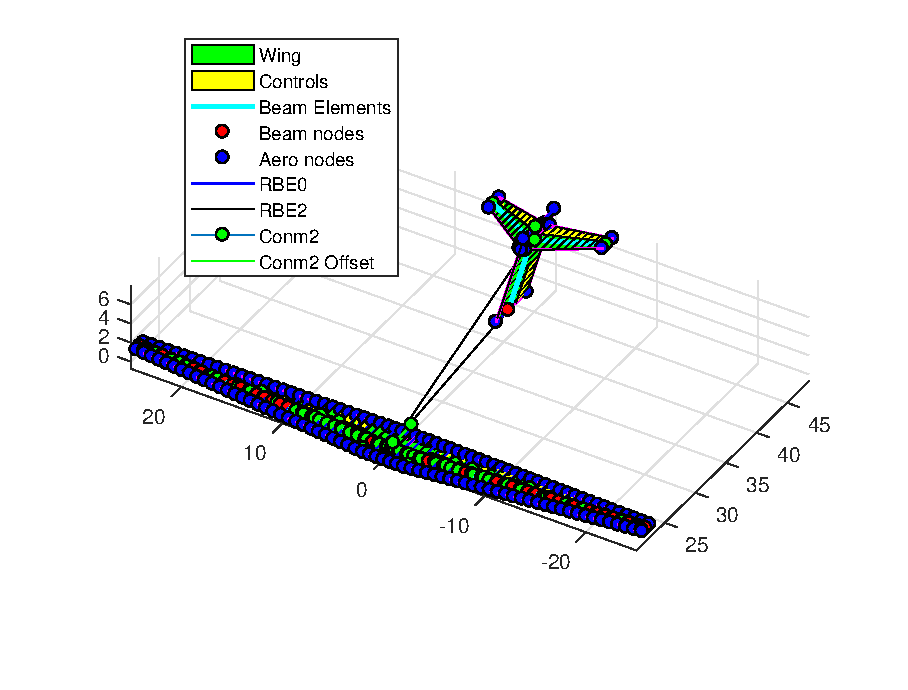
\includegraphics[width = 0.85\textwidth]{ReflectedModel}
\caption{Complete aeroelastic model of the full FAME aircraft}\label{fig:ReflectedModel}
\end{figure}

\begin{figure}[h!]
\centering
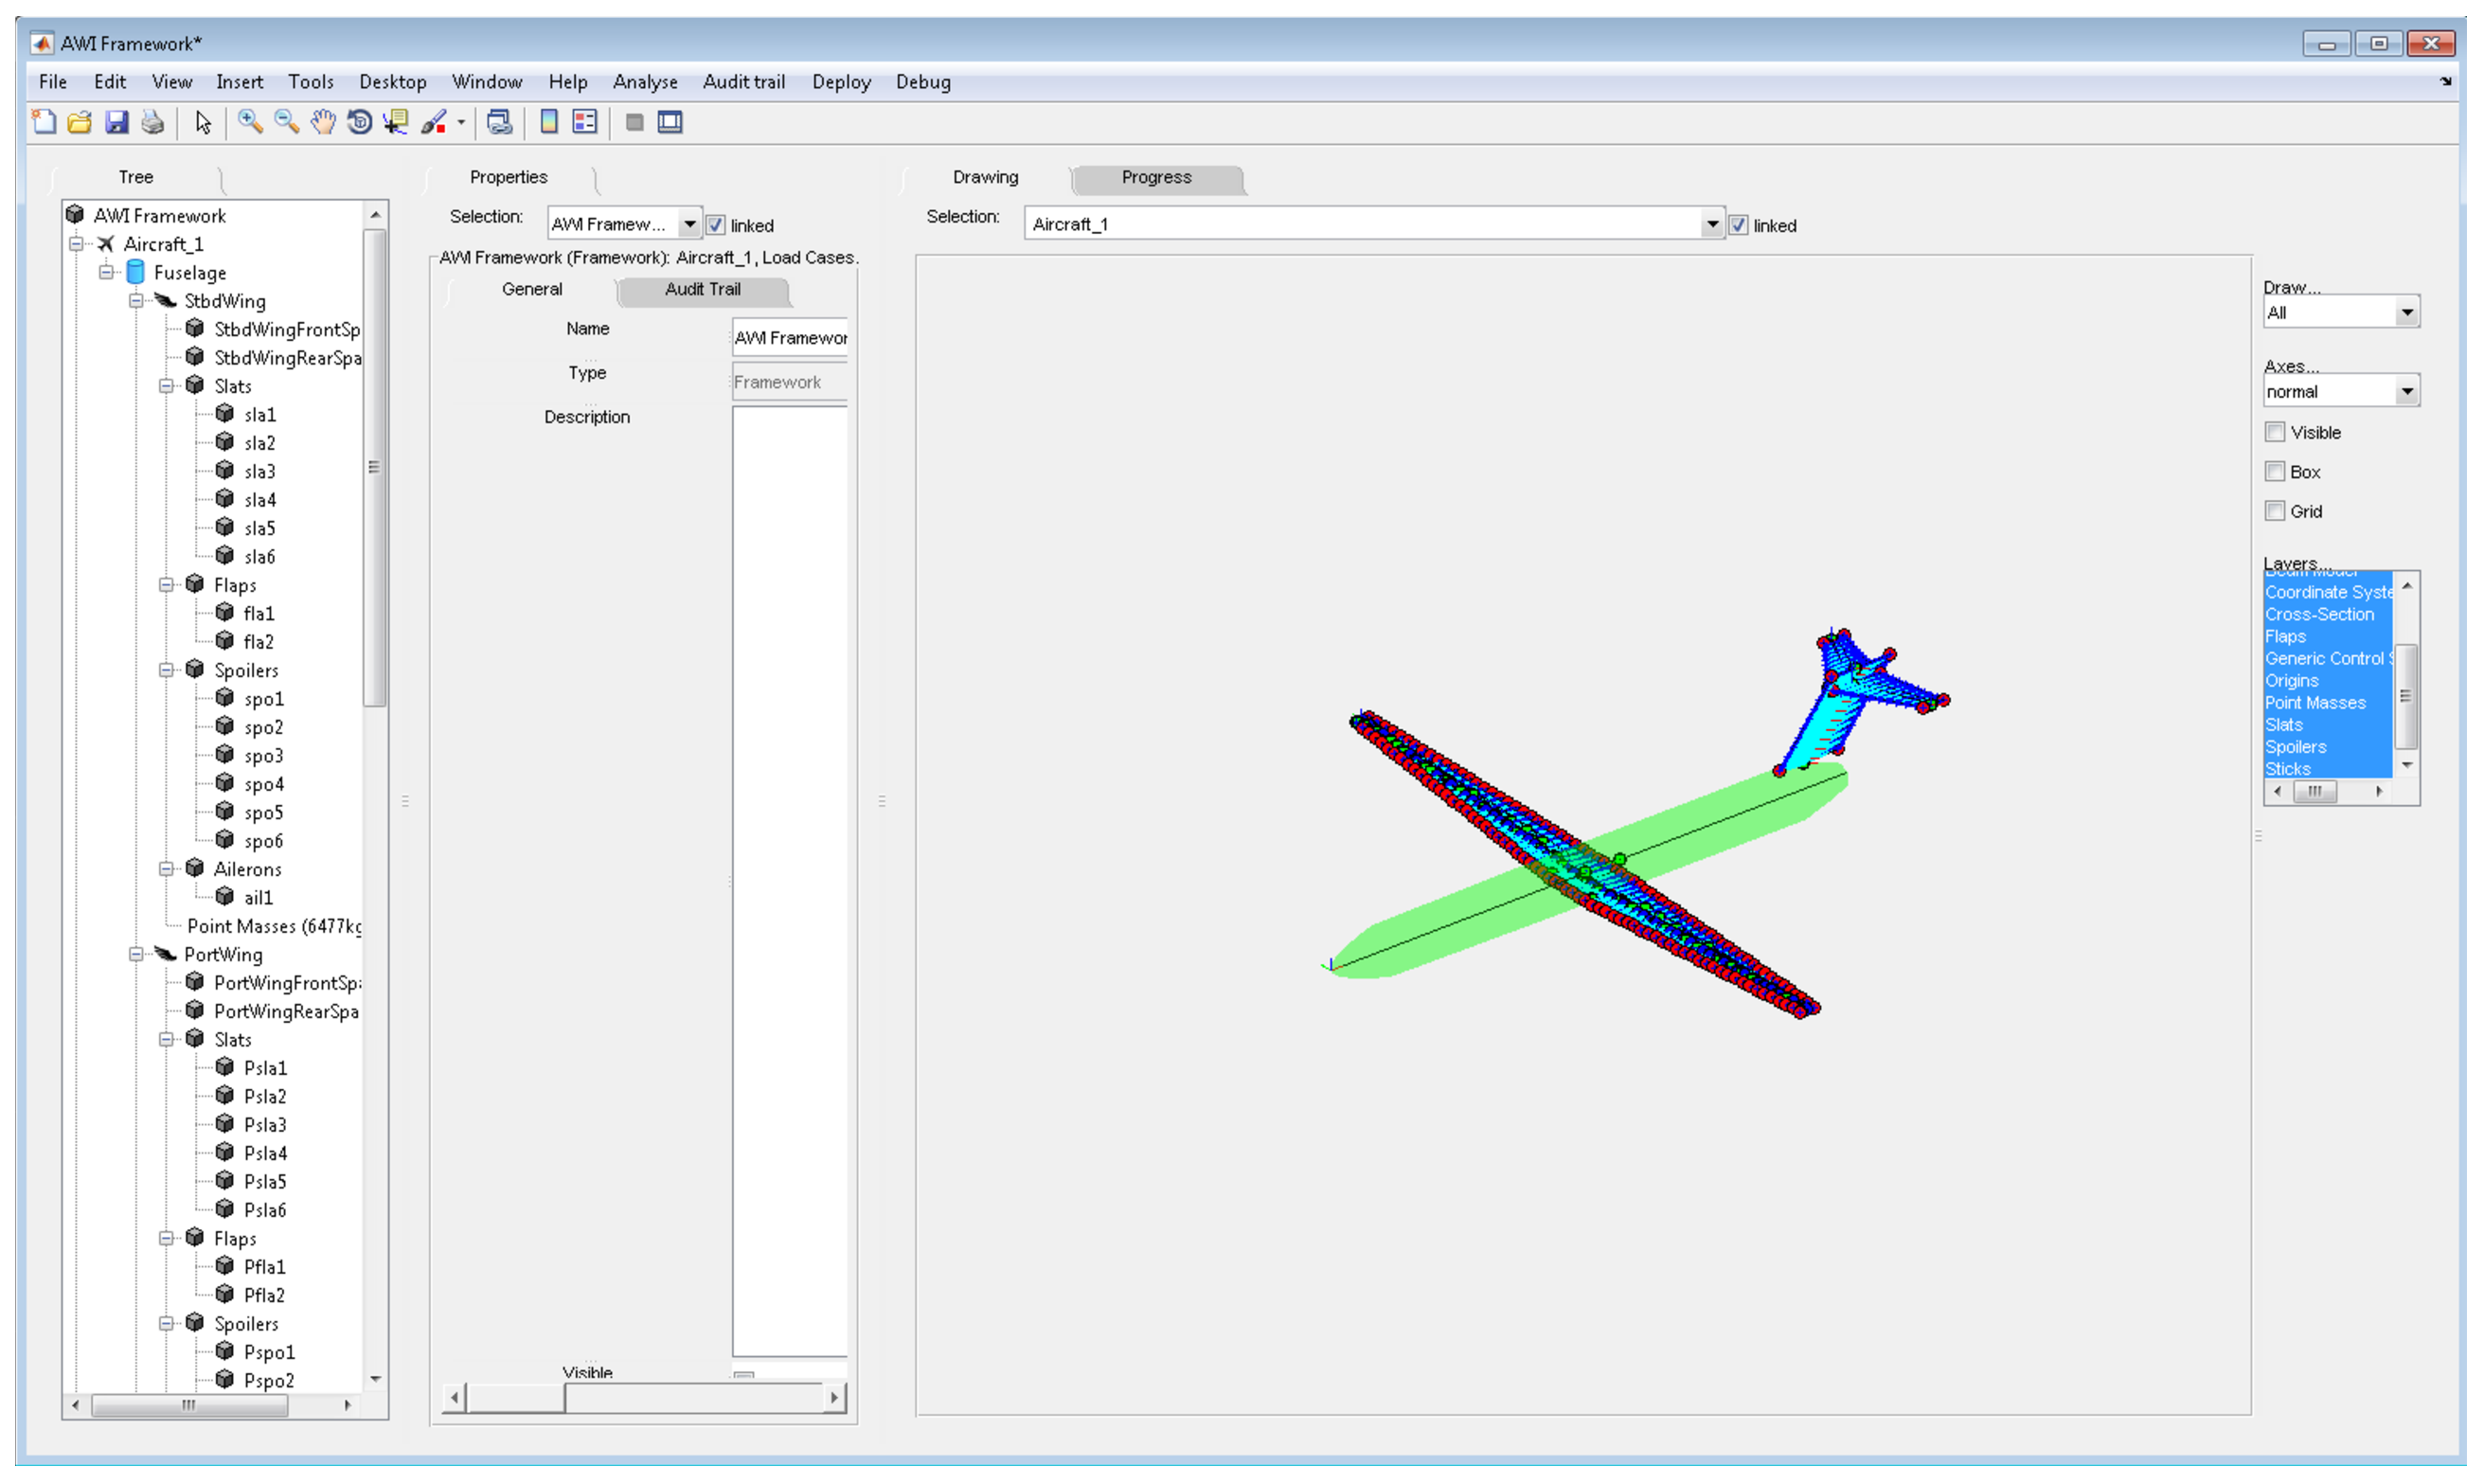
\includegraphics[width = 0.85\textwidth]{FAMEModelFramework}
\caption{Graphical representation of the FAME aircraft/beam model through the AWI GUI}\label{fig:FAMEModelFramework}
\end{figure}

\end{enumerate}



\end{document}
